\documentclass[11pt,a4paper]{article}

\usepackage[margin=2.3cm]{geometry}
\usepackage{amsmath,amssymb}
\usepackage{graphicx}
\usepackage{booktabs}
\usepackage{array}
\usepackage{xcolor}
\usepackage{enumitem}
\usepackage[hidelinks]{hyperref}
\usepackage{caption}

\emergencystretch=1.5em
\captionsetup{font=small,labelfont=bf,width=.92\textwidth}

\setlength{\parskip}{4pt plus 1pt}
\setlength{\parindent}{0pt}

\newcommand{\code}[1]{\texttt{#1}}
\newcommand{\neff}{n_{\mathrm{eff}}}
\newcommand{\chigeo}{\chi_{\mathrm{geo}}}
\newcommand{\EMA}{\operatorname{EMA}}
\newcommand{\died}[1]{\textcolor{red!70!black}{\textbf{#1}}}
\newcommand{\ok}{\checkmark}
\newcommand{\fail}{\texttimes}

\title{
Investigation of RBLapSum \code{through\_rank\_kappa} instability\\[2pt]
\large Research notebook
}

\author{}
\date{Started 2026-09-16. Investigation initiated after the France kappa campaign.}

\begin{document}

\maketitle
\vspace{-2em}
\tableofcontents


% ============================================================
\section{The question}
% ============================================================

The \code{through\_rank\_kappa} gradient mode resolved the severe instability
previously observed with \code{through\_rank}
(see \code{docs/figures/rb\_divergence\_*.png}).
At \(K=32\), \(T=1.0\), it is currently the best-performing method in the
campaign: validation CE reaches 1.491 at \(J=480\), compared with the previous
LapSum best of 1.545.

However, the campaign revealed three classes of instability that were not
initially understood:

\begin{center}\small
\begin{tabular}{p{4.2cm}p{9.6cm}}
\toprule
observation & detail \\
\midrule

\textbf{\(K=64,\ J=448,\ T=1.0\) diverges}
&
The run is healthy at 2k steps (probe-batch CE 1.81), begins to destabilize
around 3--4k steps (CE 5.9 at 4k), and is fully collapsed by 10k.
The otherwise identical \(T=2.0\) run remains healthy and finishes at 1.472.
At \(K=64,\ T=1.0\), the \(J=64\) and \(J=192\) runs are also stable.
\\[2pt]

\textbf{\(T=0.5\) at \(K=32\) is usually unstable}
&
\(J=32,96,480\) collapse. \(J=224\) survives, with a modest degradation:
1.5125 compared with 1.4940 at \(T=1\).
\\[2pt]

\textbf{\(T=0.1\) at \(K=32\) is always unstable}
&
All four tested \(J\) values diverge, with final CE around 6 or worse.
\\

\bottomrule
\end{tabular}
\end{center}

The goals of this investigation are:

\begin{enumerate}[leftmargin=1.6em]
    \item identify the mechanism responsible for the instability;
    \item determine whether the \(K\)-axis failure
    (\(K:32\to64\) at fixed \(T=1\))
    and the temperature-axis failure
    (\(T:1\to0.5\to0.1\) at fixed \(K=32\))
    arise from the same mechanism;
    \item derive a principled rule for choosing \(T\), or modify the algorithm
    so that the unstable regime is avoided automatically.
\end{enumerate}


% ============================================================
\section{Plain-language glossary}
% ============================================================

\begin{itemize}[leftmargin=1.4em]

\item \textbf{Score.}
For AbsTopK,
\[
s_i = |z_i|.
\]
The score measures the magnitude of feature \(i\) at a given token.
The gate keeps the \(K\) largest features active and additionally tracks the
next \(J\) features as backward-pass candidates.

\item \textbf{Boundary.}
\[
b = \max\left(0.1,\ s_{(K+1)}\right).
\]
Here \(s_{(K+1)}\) is the score of the first inactive feature.
Thus \(b\) is the local threshold separating the active support from the
inactive candidate region.

\item \textbf{Kernel.}
\[
\kappa_T(s-b)
=
\frac{e^{-|s-b|/T}}{2T}.
\]
This is an exponential kernel centered at the boundary.
The surrogate support gradient is weighted by \(\kappa_T\), so features near
the boundary receive the strongest support-learning signal.

Its characteristic width is \(T\), while its maximum value is
\[
\kappa_{\max}=\frac{1}{2T}.
\]
Reducing \(T\) therefore makes the kernel narrower and increases its peak
magnitude.

\item \textbf{Raw surrogate term.}
\[
a_i = u_i z_i \kappa_i,
\qquad
u_i = \frac{\partial L}{\partial y_i}.
\]
Here \(u_i\) is the ordinary task-loss gradient arriving at the bottleneck
output. The quantity \(a_i\) is the independent local contribution that would
be obtained before applying the collective correction.

\item \textbf{Kappa correction.}
\[
g_i
=
a_i - q_i \sum_j a_j,
\qquad
q_i
=
\frac{\kappa_i}{\sum_j \kappa_j}.
\]
The correction removes the collective score-gradient component while
distributing the compensating term among candidates in proportion to their
kernel weights.

This distinguishes \code{through\_rank\_kappa} from \code{detach}, where no
collective correction is applied.

\item \textbf{Feature preference signal.}
Define
\[
w_i=-u_i z_i.
\]
With this sign convention, \(w_i>0\) means that the task loss locally prefers
feature \(i\) to contribute more strongly.

A gradient-descent step in score space has the schematic form
\[
\Delta s_i
\propto
\kappa_i
\left(
w_i-\langle w\rangle_q
\right),
\]
where
\[
\langle w\rangle_q
=
\sum_i q_i w_i.
\]
Thus a near-boundary feature moves upward when it is preferred more strongly
than the kernel-weighted local average, and downward when it is preferred less.

\item \textbf{Local spacing.}
Let
\[
\delta(b)
=
\frac{s_{(K-3)}-s_{(K+5)}}{8}.
\]
This estimates the typical spacing between neighboring feature ranks near the
boundary. Small \(\delta\) means that many features occupy a narrow score
interval around the support threshold.

\item \textbf{Effective window population.}
\[
\neff
=
\frac{\left(\sum_i\kappa_i\right)^2}
{\sum_i\kappa_i^2}.
\]
This is an effective-number-of-elements measure for the kernel weights. It
estimates how many candidates meaningfully participate in the local boundary
correction.

\end{itemize}


% ============================================================
\section{What we know going in}
% ============================================================

\begin{itemize}[leftmargin=1.4em]

\item Previous analysis of \code{through\_rank}, where the entire boundary
correction is assigned to the single \((K+1)\)-st feature, identified the
following failure mode: the boundary feature can receive an anomalously large
update; activation scale then grows through depth along weakly constrained
scale directions; the boundary eventually moves far outside the kernel region;
the support gradient vanishes; and optimization becomes trapped at a very
large activation scale.

\item \code{detach}, which applies no collective correction, was stable for
20k steps at \(K=32,\ T=1.0\). Thus a collective correction is not required for
stability in that particular regime.

\item The \(K=64\) campaign shares the same architecture and training setup as
the \(K=32\) runs except for \(K\) and \(J\):
\(8\times768\), MD/decouple, \code{abs\_topk}, \code{residual\_out},
\(b_0=0.1\), and the same learning-rate schedule.

\item
\code{uk\_rout\_rblapsum\_kappa\_k64\_j448\_md\_abs}
and
\code{...k32\_j480...}
both track 512 features in total.
The main structural difference is therefore the location of the support
boundary: rank 65 versus rank 33.
This suggests that the local score geometry at the boundary, rather than the
total number of candidates alone, may be important.

\end{itemize}


% ============================================================
\section{Candidate mechanisms}
% ============================================================

The following hypotheses were formulated before the detailed measurements.

\subsection*{H1 --- Degeneration of the kappa correction}

As \(T\to0\), the kernel weights may become concentrated on only one or a few
features near the boundary. In the extreme case,
\[
\neff\to1,
\]
and the distributed correction approaches the original
\code{through\_rank} behavior, where the collective correction is effectively
carried by a single feature.

Prediction:
instability should correlate with small \(\neff\).

A difficulty for this hypothesis is the \(K\)-dependence.
At fixed \(T\), the rank-65 boundary lies in a denser part of the score
distribution than rank 33. One might therefore initially expect a larger,
not smaller, \(\neff\) at \(K=64\).

\subsection*{H2 --- Excessive surrogate-force magnitude}

The maximum per-candidate kernel weight is
\[
\kappa_{\max}
=
\frac{1}{2T}.
\]

If the local score density is
\[
\rho(b)\approx\frac{1}{\delta(b)},
\]
then for the exponential kernel,
\[
\sum_i \kappa_i^2
\approx
\frac{\rho(b)}{4T}.
\]

Thus reducing \(T\) increases both the peak local gradient and the total
squared surrogate weight in the boundary region.

This hypothesis qualitatively explains both observed axes:

\[
T\downarrow
\quad\Rightarrow\quad
\text{stronger kernel},
\]

and

\[
K\uparrow
\quad\Rightarrow\quad
\text{potentially larger local density } \rho(b).
\]

The main quantitative question is whether the measured change in local density
is large enough to account for the \(K=32\to64\) transition.

\subsection*{H3 --- Boundary churn and cumulative scale drift}

Define a dimensionless comparison between the characteristic surrogate-induced
score displacement and the local spacing between ranks:

\[
\chi
=
\frac{
\text{characteristic boundary-region score displacement}
}{
\delta(b)
}.
\]

The intended interpretation is that when the surrogate moves near-boundary
features by an amount comparable to their rank spacing, the identities of
near-boundary features can change rapidly from step to step.

A possible cumulative mechanism is then:

\begin{enumerate}[leftmargin=1.6em]
    \item the correction is zero-sum within the current candidate set;
    \item a feature pushed upward can leave the boundary region and retain its
    increased score;
    \item a feature pushed downward can leave the candidate set or move to a
    region with negligible kernel weight;
    \item consequently, exact cancellation at one instant does not necessarily
    imply cancellation over a sequence of changing candidate sets.
\end{enumerate}

This can create a small systematic bias in score dynamics even when each
individual correction is zero-sum.

Using the rough local scale
\[
\text{kick}
\sim
\frac{\eta |u| b}{2T},
\]
one obtains
\[
\chi
\propto
\frac{\eta |u| b}{2T\,\delta(b)}.
\]

This predicts instability when the boundary region is simultaneously:
\begin{itemize}[leftmargin=1.4em]
    \item sharply weighted by the kernel (\(T\) small),
    \item located at large score scale \(b\),
    \item and densely populated (\(\delta\) small).
\end{itemize}

It also predicts weak direct dependence on \(J\) at fixed local geometry.

\subsection*{H4 --- Switching between rank and floor regimes}

Because
\[
b=\max(b_0,s_{(K+1)}),
\]
it is possible in principle that deeper boundaries, such as \(K=64\), cross
the floor \(b_0=0.1\). This would switch the backward rule between a
rank-dependent and a fixed-boundary regime.

This hypothesis can be tested directly using
\code{rb\_cap\_active\_frac}.

\subsection*{Relation between H2 and H3}

H2 and H3 are closely related.
Both propose that the kernel becomes too strong relative to the local score
geometry.

H3 is more specific because it introduces the local rank spacing as the
comparison scale and proposes a dynamical mechanism by which repeated
near-boundary updates can accumulate.

H1 concerns a different limit: the distributed correction itself ceases to be
distributed once the effective kernel population becomes very small.


% ============================================================
\section{Evidence plan}
% ============================================================

\begin{enumerate}[leftmargin=1.6em]

\item \textbf{Run outcomes and onset timing.}

Use the France TensorBoard scalars
(\code{analysis/kappa\_stability.py tb}) to determine when each run
destabilizes and whether
\code{rb\_support\_grad\_norm},
\code{rb\_boundary}, or
\code{rb\_cap\_active\_frac}
changes first.

\item \textbf{Score geometry.}

Use the \code{lens\_1} score ladders
(\code{... ladder}) to measure
\[
\delta,\qquad
b,\qquad
\sum_i\kappa_i,\qquad
\neff
\]
for each layer and checkpoint.

Measure these both at each run's actual boundary and counterfactually at ranks
33 and 65 in the same activation tensors. This isolates the geometric effect
of moving the boundary deeper into the same score distribution.

\item \textbf{Training-time surrogate forces.}

Use probe captures
(\code{... probe}) to reconstruct
\[
a,\qquad q,\qquad g_s
\]
from captured \((z,u)\), and verify the reconstruction against the captured
gradient with respect to \(z\).

Measure:
\begin{itemize}[leftmargin=1.4em]
    \item local surrogate-gradient magnitudes;
    \item \(\operatorname{Cov}_q(d,w)\), which characterizes stretching or
    compression of the boundary band;
    \item support churn between probes;
    \item cumulative asymmetries in how upward- and downward-moving candidates
    leave the kernel region.
\end{itemize}

\item \textbf{Falsification runs.}

Use the available France \(8\times5090\) machine to test predictions that
distinguish the candidate mechanisms.

\end{enumerate}


% ============================================================
\section{Evidence phase 1: outcomes, onset, and early indicators}
% ============================================================

The following results were extracted with
\code{analysis/kappa\_stability.py tb} from the France TensorBoard logs.

The reported onset is the first step whose training loss exceeds the best loss
so far by 1 nat.

\begin{table}[h]
\centering
\small

\begin{tabular}{rrrrr@{\hskip 2em}rrrrr}
\toprule
\(K\) & \(J\) & \(T\) & onset & final CE &
\(K\) & \(J\) & \(T\) & onset & final CE \\
\midrule

32 & 32  & 0.1 & 640  & 5.98 &
32 & 32  & 1.0 & ---  & 1.548 \\

32 & 96  & 0.1 & 640  & 9.44 &
32 & 96  & 1.0 & ---  & 1.525 \\

32 & 224 & 0.1 & 520  & 5.98 &
32 & 224 & 1.0 & ---  & 1.494 \\

32 & 480 & 0.1 & 580  & 5.98 &
32 & 480 & 1.0 & ---  & 1.491 \\

32 & 32  & 0.5 & 3760 & 6.08 &
\multicolumn{2}{r}{32--64, all} & 2.0 & --- & 1.47--1.56 \\

32 & 96  & 0.5 & 6480 & 5.53 &
64 & 64  & 1.0 & ---  & 1.504 \\

32 & 224 & 0.5 & --- & 1.512 &
64 & 192 & 1.0 & --- & 1.489 \\

32 & 480 & 0.5 & 7760 & 5.77 &
64 & 448 & 1.0 & \died{3940} & 14.04 \\

\bottomrule
\end{tabular}

\caption{Outcomes of the 22 campaign runs. ``---'' indicates survival through
20k training steps.}
\end{table}


\begin{figure}[h]
\centering
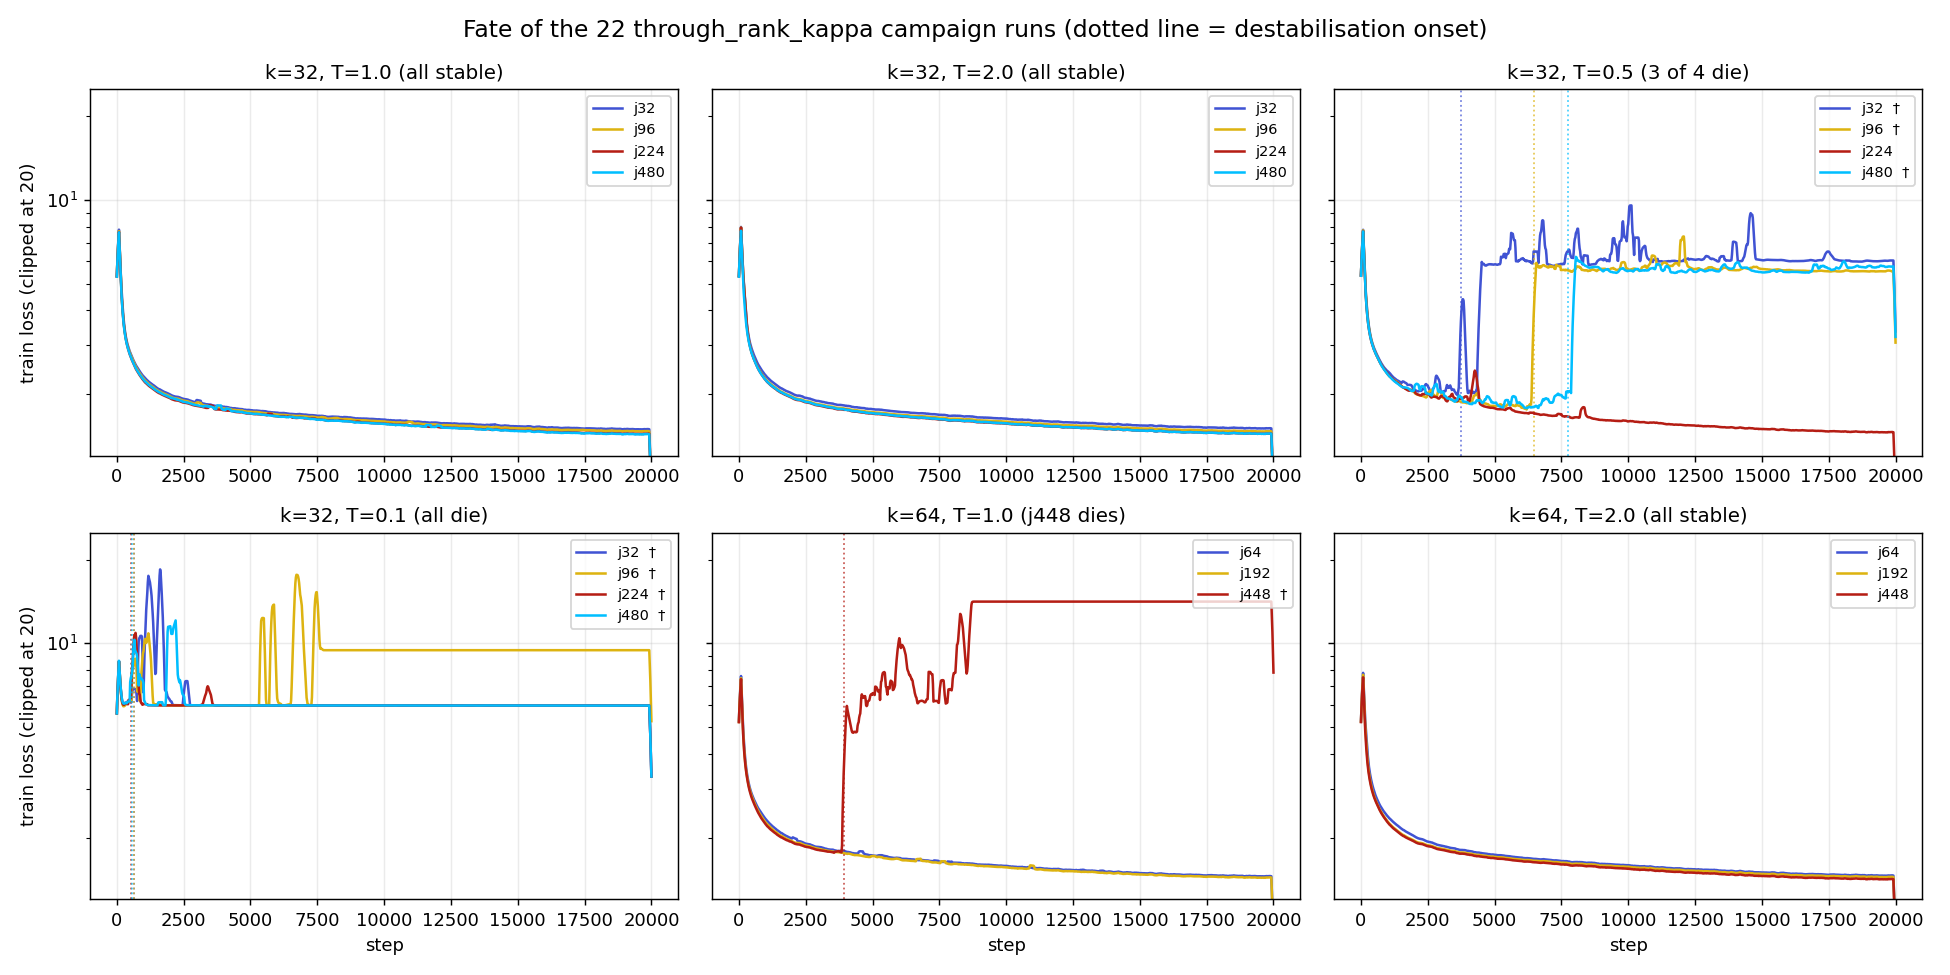
\includegraphics[width=\textwidth]{figures/kstab_fate_grid.png}
\caption{Training-loss outcomes for the 22
\code{through\_rank\_kappa} campaign runs. Dotted lines indicate the measured
destabilization onset.}
\end{figure}

Several observations from the TensorBoard signals are particularly useful.

\begin{itemize}[leftmargin=1.4em]

\item
\code{rb\_cap\_active\_frac} remains \(1.0\) throughout all runs, including
during collapse.

Therefore the \(b_0\) floor is not active in the observed failures, which rules
out H4 for this campaign.

\item
\code{rb\_common\_mode} remains around \(10^{-6}\).

Thus the kappa correction continues to remove the collective score-gradient
component accurately even while the model destabilizes. The failure is not
caused by a simple numerical loss of the zero-sum property.

\item
The boundary score \(b\) begins to increase substantially before the task loss
shows visible deterioration.

For the unstable \(T=0.5\) runs, \(b\) can remain between 25 and 500 times its
baseline value for hundreds or thousands of steps before the measured onset.

For \(K=64,\ J=448,\ T=1\), the last 1000 steps before onset show approximately
a 22\% increase in \(b\) and a 4.4-fold increase in gradient norm.

\item
\code{rb\_support\_grad\_norm} does not show a smooth pre-onset divergence.

The surrogate support gradient therefore does not simply explode first and
directly drive the task loss upward.
Instead, the available evidence is more consistent with the surrogate slowly
moving the model into an unstable part of parameter/activation space, after
which the ordinary task gradients become large.

\end{itemize}


\begin{figure}[h]
\centering
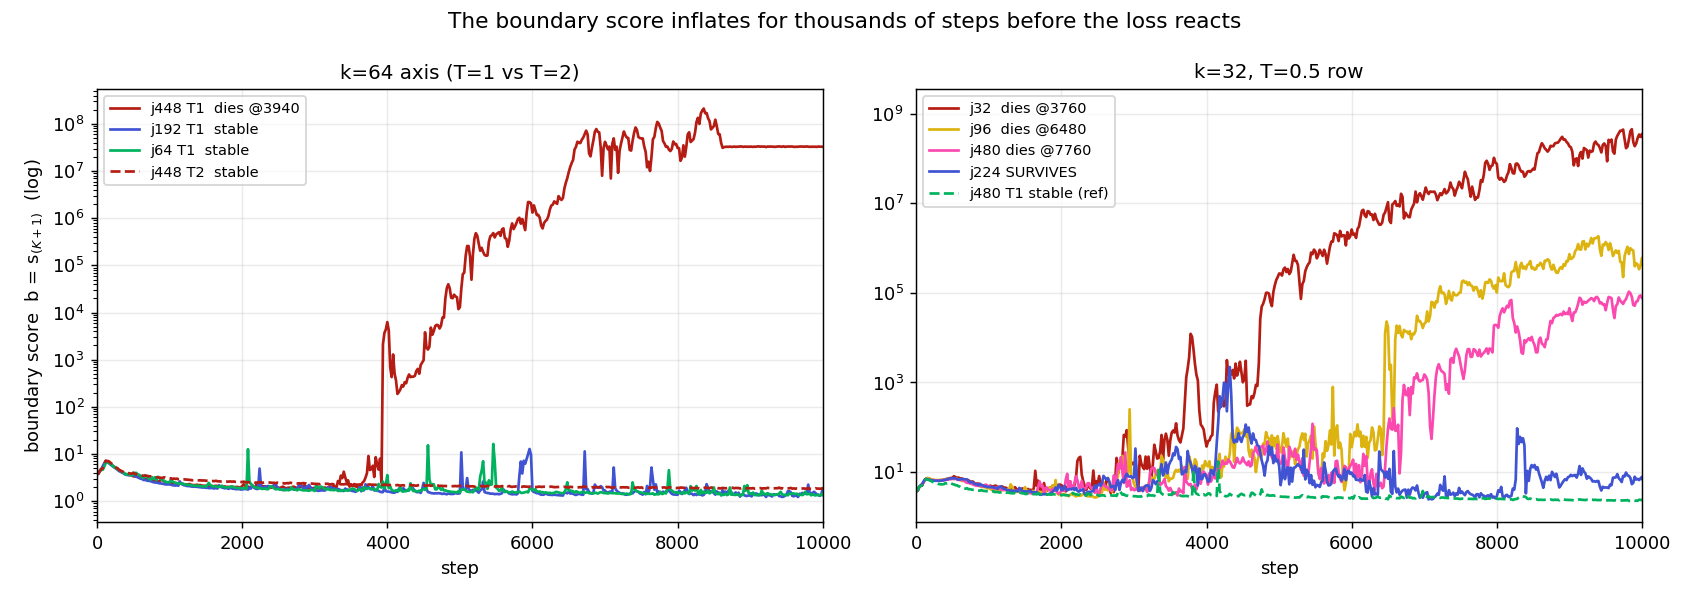
\includegraphics[width=\textwidth]{figures/kstab_boundary_inflation.png}
\caption{
Boundary-score inflation can precede visible loss degradation by hundreds or
thousands of training steps.
Left: the \(K=64\) comparison.
Right: the \(K=32,\ T=0.5\) runs.
}
\end{figure}

A further observation changes the picture from a simple monotonic drift to a
metastable process.

Marginal runs show repeated transient excursions of the boundary score, often
followed by recovery. In some cases the excursions reach factors of
\(10^2\)--\(10^3\) relative to the local baseline.

For example, the surviving \(K=32,\ J=224,\ T=0.5\) run undergoes two
approximately \(10^3\)-fold excursions near step 4300 and recovers from both.

In unstable runs, the final failure appears to correspond to an excursion from
which the system does not recover, followed by persistent scale growth.

For clarity, we refer to these transient excursions as \emph{inflation bursts}.

The table below counts excursions for which \(b\) exceeds three times its
rolling median, normalized per 1000 pre-onset steps.

\begin{center}\small
\begin{tabular}{lll}
\toprule
configuration & burst rate & outcome \\
\midrule

\(K=32,\ T=2\) and \(K=64,\ T=2\)
&
0.00
&
all stable; maximum excursion \(\le1.9\times\)
\\

\(K=32,\ T=1\)
&
0.05--0.21
&
all stable
\\

\(K=64,\ T=1\)
&
\(J64:0.37,\ J192:0.42,\ \mathbf{J448:0.97}\)
&
\(J448\) diverges
\\

\(K=32,\ T=0.5\)
&
\(J224:\mathbf{0.52},\ J480:1.7,\ J32:3.1,\ J96:3.2\)
&
\(J224\) is the only survivor
\\

\bottomrule
\end{tabular}
\end{center}

Within these rows, burst rate is associated with outcome:
the unstable \(K=64\) run has the highest burst rate in its row, while the
surviving \(T=0.5\) run has the lowest rate by a factor of roughly 3--6.

This does not by itself establish a causal role for burst rate, but it provides
a useful empirical marker for proximity to the unstable regime.


% ============================================================
\section{Evidence phase 2: measured surrogate forces}
% ============================================================

The command
\code{analysis/kappa\_stability.py probe}
reconstructs the surrogate gradient per candidate from probe captures using
\[
u=\frac{\partial L}{\partial \tilde z}
\]
together with the signed \(z\).

The reconstruction agrees with the captured
\[
\frac{\partial L}{\partial z}
\]
to approximately zero relative error at the reported precision, so the
quantities below correspond to the actual training-time backward rule.

\subsection*{The \(T=0.1\) collapse}

Consider \(K=32,\ J=96,\ T=0.1\), layer 4.

Here ``kick'' denotes the mean \(|g_s|\) among candidates in the kernel region,
and \(\neff\) measures the effective number of candidates sharing that region.

\begin{center}\small
\begin{tabular}{rrrrrr}
\toprule
step & probe CE & kick & \(\neff\) & \(s_{(K+1)}\) & top-\(K\) mean \\
\midrule

0    & 11.30 & \(7.2\cdot10^{-3}\) & 22 & 3.8   & 4.3 \\
100  & 7.18  & \(5.7\cdot10^{-5}\) & 15 & 4.9   & 5.7 \\
150  & 6.20  & \(1.9\cdot10^{-4}\) & 3  & 11.9  & 15.6 \\
250  & 6.10  & \(6.1\cdot10^{-4}\) & 2  & 36    & 47 \\
350  & 5.84  & \(1.7\cdot10^{-6}\) & \textbf{1} & 50 & 73 \\
500  & 6.06  & \(\sim0\) & 1 & 664 & 1297 \\
1000 & 17.2  & \(\sim0\) & 1 & 21941 & 49688 \\

\bottomrule
\end{tabular}
\end{center}

The observed sequence is:

\begin{enumerate}[leftmargin=1.6em]

\item The initial kernel is very sharp:
\[
\kappa_{\max}
=
\frac{1}{2T}
=
5.
\]

\item Scores begin to increase and move away from the original boundary region.

\item The effective kernel population falls:
\[
\neff:22\to15\to3\to2\to1.
\]

\item Once \(\neff\approx1\), the distributed kappa correction effectively
approaches the single-boundary-feature limit of
\code{through\_rank}.

\item Activation scale then increases rapidly.

\item Eventually the candidates move so far from the kernel that the support
gradient itself becomes nearly zero.

\item At that stage the model remains at an activation scale several orders of
magnitude above the initial regime, while the task loss is badly degraded.

\end{enumerate}

The support dynamics change correspondingly.
At the beginning of the run, approximately 96\% of the top-\(K\) support is
replaced over 10 steps, compared with roughly 30\% in healthy runs.
Later, after the activation scale has become very large, the support freezes
and the overlap approaches 1.


% ============================================================
\subsection*{A kick-to-spacing diagnostic}
% ============================================================

Define

\[
\chi
=
\frac{
\overline{|g_s|}_{\mathrm{window}}
}{
\delta(b)
}.
\]

This quantity compares the surrogate gradient scale near the boundary with the
local score spacing.

Strictly speaking, the expression above is in gradient units rather than
literal per-optimizer-step displacement units.
A true displacement criterion would also depend on the optimizer and effective
step size.
Nevertheless, when computed under the same training setup, this quantity is
useful for comparing runs.

Measured over steps 300--1000:

\begin{center}\small
\begin{tabular}{lll}
\toprule
configuration & \(\chi\) (layer mean) & outcome \\
\midrule

\(K=32,\ T=2\)
&
\(2.7\cdot10^{-5}\)
&
stable
\\

\(K=64,\ T=2\)
&
\(5.4\cdot10^{-5}\)
&
stable
\\

\(K=32,\ T=1\)
&
\(8.2\cdot10^{-5}\)
&
stable
\\

\(K=64,\ T=1\)
&
\(1.5\)--\(1.7\cdot10^{-4}\), similar across all three \(J\)
&
marginal; 1 of 3 diverges
\\

\(K=32,\ T=0.5\)
&
\(1.9\cdot10^{-4}\)
&
marginal; 3 of 4 diverge
\\

\(K=32,\ T=0.1\)
&
\(\sim10^{-2}\) at initialization
&
diverges within several hundred steps
\\

\bottomrule
\end{tabular}
\end{center}

Within the measured campaign, \(\chi\) is primarily a property of the
\((K,T)\) row and varies little with \(J\).

The empirical ordering is:

\[
\text{stable regime}
\quad\lesssim\quad
10^{-4},
\]

\[
\text{marginal regime}
\quad\sim\quad
1.5\text{--}2\times10^{-4},
\]

while \(T=0.1\) begins roughly two orders of magnitude above these values.

The measured scaling is consistent with

\[
\chi
\propto
\frac{|u|\,b}
{2T\,\delta(b)}.
\]

The boundary at rank 65 lies in a substantially denser score region than the
boundary at rank 33.
Measured inside the same activation tensors,
\[
\frac{\delta_{33}}{\delta_{65}}
\approx
3.3\text{--}4.6.
\]

The rank-65 boundary also has approximately 30\% smaller \(b\).
Combining these effects gives

\[
\frac{
\chi(K=64,T=1)
}{
\chi(K=32,T=1)
}
\approx
2.2,
\]

which is close to

\[
\frac{
\chi(K=32,T=0.5)
}{
\chi(K=32,T=1)
}.
\]

Thus, with respect to this local pressure measure,

\[
K=64,\ T=1
\]

is approximately comparable to

\[
K=32,\ T\approx0.5.
\]

The measured ratio of safe temperatures,
\[
\frac{T_c(64)}{T_c(32)}
\approx2.2,
\]
is consistent with the observation that \(T=2\) is stable at \(K=64\).

This supports the hypothesis that the \(K\)-axis and \(T\)-axis failures arise
from the same underlying interaction between kernel width and local score
geometry.


% ============================================================
\subsection*{Two additional observations}
% ============================================================

\begin{itemize}[leftmargin=1.4em]

\item
In healthy steady states,
\[
\neff\approx46\text{--}446,
\]
far from the \(\neff\approx1\) regime.

Thus H1 does not explain the ordinary operating state.
Instead, degeneration of the correction appears to occur only during severe
inflation episodes and may act as a terminal amplification mechanism once the
window has already collapsed.

\item
A small cumulative asymmetry is measurable even in healthy runs.

Candidates receiving upward surrogate updates fall approximately 0.04 score
units less over 10 steps than candidates receiving downward surrogate updates,
against a mean regression of approximately \(-0.5\).

Thus the surrogate contributes only a few percent bias to the background score
dynamics in the healthy regime.
This is consistent with a gradual modification of the score distribution
rather than direct domination of the optimizer.

\end{itemize}


% ============================================================
\section{Theory v3: burst-driven escape}
% ============================================================

The evidence above suggests the following working model.

\begin{enumerate}[leftmargin=1.6em]

\item
The kernel applies persistent pressure to the boundary region.
The relevant strength is controlled by the kernel scale relative to the local
score geometry, summarized empirically by \(\chi\).

\item
The network can partially accommodate this pressure by changing the overall
score scale.
As the scale increases, fewer candidates remain strongly weighted by the
fixed-width kernel.
The ordinary task loss provides an opposing force.

\item
At low enough pressure, these effects remain in a stable regime.
This is consistent with the absence of bursts at \(T=2\) and the low burst
rate at \(K=32,T=1\).

\item
In the marginal regime, transient score-inflation excursions become more
frequent.

\item
If an excursion reduces the effective kernel population to
\[
\neff=O(1),
\]
the distributed kappa correction approaches its single-feature
\code{through\_rank} limit.

Previous experiments indicate that this limit strongly favors further
activation-scale growth.

\item
The excursion can then become self-sustaining:
the score scale increases, the kernel population shrinks further, and
eventually the support gradient itself becomes negligible because almost all
features lie far outside the kernel.

The model is then left in a high-activation-scale state with poor task loss.

\item
At \(T=0.1\), this sequence occurs reproducibly within the first few hundred
steps.

At intermediate pressures, failure is stochastic:
individual runs may undergo several recoverable bursts before one becomes
unrecoverable.

\end{enumerate}


% ============================================================
\section{Falsification wave 1}
% ============================================================

These runs use 6k-step observations within the same 20k-step training
schedules.

The following predictions were recorded before the runs.

\begin{center}\small
\begin{tabular}{p{3.6cm}p{4.4cm}p{5.6cm}}
\toprule
run & question & prediction under theory v3 \\
\midrule

\(K64,J448,T1\) \textbf{detach}
&
Is the kappa correction itself responsible for the failure?
&
If the raw kernel force is the main source of the scale pressure, detach
should also be unstable at this operating point.
\\

\(K64,J448,T1\) \textbf{project}
&
Does uniform common-mode removal behave differently from kappa-weighted
removal?
&
Expected behavior between detach and kappa.
\\

\(K64,J448,T1\), seed 1338
&
Is the failure at step 3940 deterministic?
&
If failure is an escape process, a different seed should have a different
onset and may survive substantially longer.
\\

\(K64,J448,T=1.5\)
&
Bracket the pressure threshold.
&
With estimated \(\chi\approx1.0\)--\(1.1\times10^{-4}\), the run should lie
near the stable edge.
\\

\(K64,J320,T1\)
&
Test the role of \(J\) within the marginal \(K64,T1\) row.
&
Since \(\chi\) is similar across the row, outcome should depend mostly on
stochastic burst occurrence rather than a deterministic \(J\) threshold.
\\

\(K32,J480,T=0.75\)
&
Bracket the threshold along the \(K32\) temperature axis.
&
Expected to be near the stable side of the marginal region.
\\

\(K32,J96,T0.5\), seed 1338
&
Test reproducibility of the unstable \(T=0.5\) regime.
&
Expected to diverge, but not necessarily at the same step as the original run.
\\

5k probe of \(K64,J448,T1\)
&
Capture gradients during a possible failure.
&
If a collapse occurs, \(\neff\) should fall strongly during the final
inflation episode.
\\

\bottomrule
\end{tabular}
\end{center}


Early observations at approximately step 1100 already showed:

\begin{itemize}[leftmargin=1.4em]

\item the \code{detach} run had CE 9.0 and infinite gradient norm;

\item the \code{project} run had CE 7.1 and infinite gradient norm;

\item the corresponding kappa-corrected runs remained healthy at the same
stage.

\end{itemize}

This is important because \code{detach} had previously been stable for 20k
steps at \(K=32,T=1\).

Thus the distributed kappa correction is not simply the source of instability.
At the higher-pressure \(K=64,T=1\) operating point it provides substantially
more protection than either detach or the uniform projection.


\begin{figure}[h]
\centering
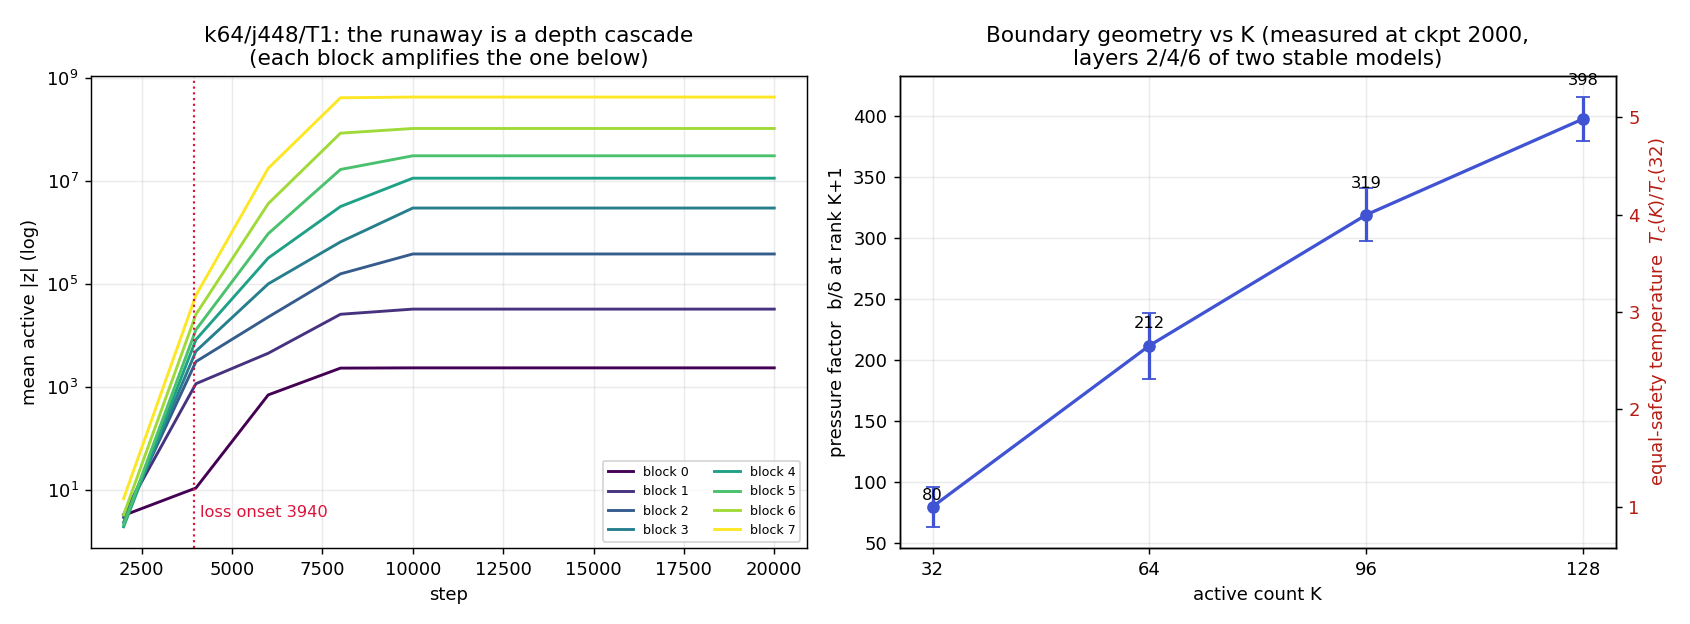
\includegraphics[width=\textwidth]{figures/kstab_cascade_and_geometry.png}
\caption{
Left: after the onset of severe instability, activation-scale growth propagates
through depth. With \code{residual\_out}, each block can amplify the scale
passed from the preceding block, eventually reaching bf16 saturation.
Right: the geometric pressure factor \(b/\delta\) grows approximately with
\(K\) over the measured range.
}
\end{figure}


\begin{figure}[h]
\centering
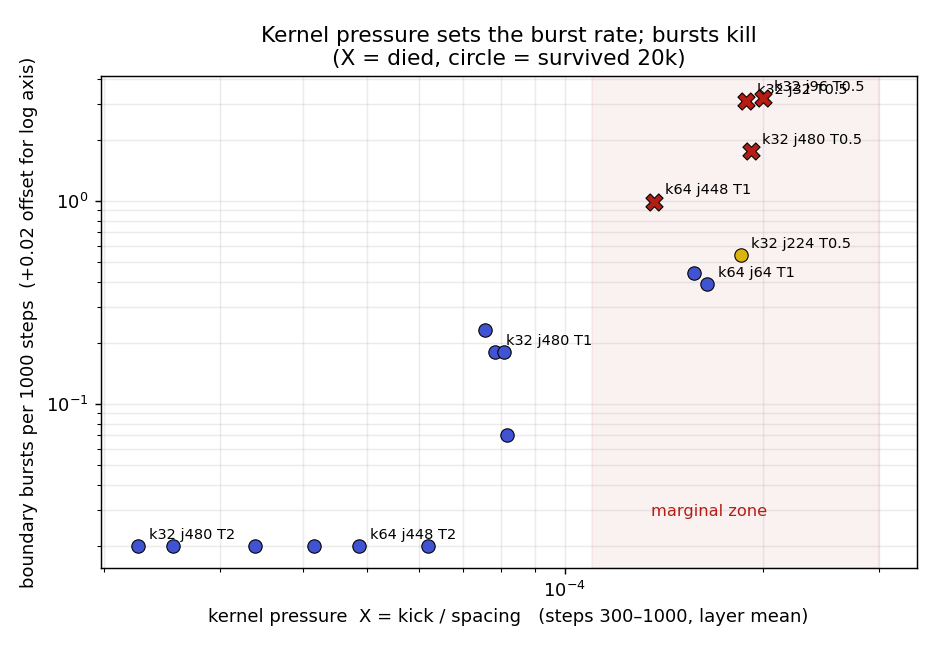
\includegraphics[width=.72\textwidth]{figures/kstab_dose_response.png}
\caption{
Observed relation between kernel-pressure diagnostics and instability.
Crosses indicate runs that diverged; circles indicate runs that survived 20k
steps.
}
\end{figure}


\begin{figure}[h]
\centering
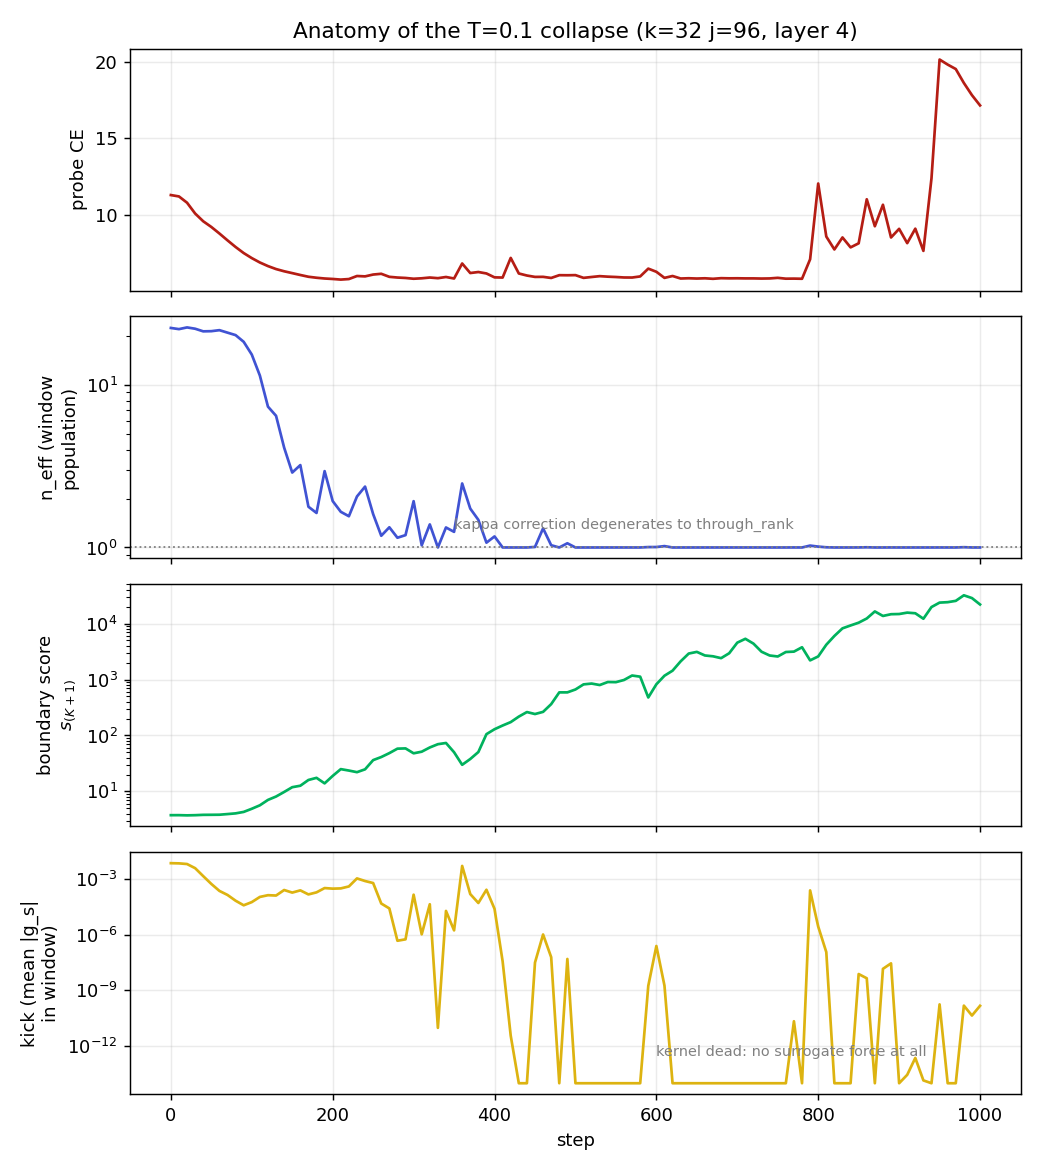
\includegraphics[width=.8\textwidth]{figures/kstab_t01_anatomy.png}
\caption{
Detailed evolution of the \(K=32,\ J=96,\ T=0.1\) collapse in layer 4.
}
\end{figure}

The \(T=0.1\) example also clarifies the ordering of events.

The effective kernel population reaches approximately one by step 350 while
the task CE is still relatively normal.
The boundary score is already increasing rapidly at this stage.
The measured support kick then falls toward zero as the kernel loses its
effective population around step 450.
The task loss does not visibly deteriorate until roughly step 800.

Thus the task loss is a delayed indicator of the underlying score-scale
instability.


% ============================================================
\section{Adaptive temperature controller: initial design}
% ============================================================

The working theory identifies two relevant conditions:

\begin{enumerate}[leftmargin=1.6em]
    \item sustained excessive kernel pressure;
    \item a sufficiently severe inflation episode that reduces the effective
    boundary population to \(O(1)\).
\end{enumerate}

Both can in principle be measured by the gate itself.
This motivates feedback control of \(T\) rather than a fixed temperature
schedule or a lookup table indexed by \(K\).

The initial implementation was

\[
\code{rblapsum\_temperature\_mode: servo}.
\]

It is implemented in
\code{src/wsparse/bottleneck/\{gate,rblapsum\}.py},
with a separate scalar \(T\) per layer stored in persistent buffers.

The first design used two mechanisms.

\subsection*{Population floor}

If fewer than
\[
\code{rblapsum\_window\_floor}=16
\]
candidates occupy the kernel window on a batch, increase \(T\) by 10\% on that
step.

The purpose is to prevent the effective boundary population from collapsing
toward the single-feature regime.

During an inflation episode, the boundary moves away from nearby candidates
and the kernel population falls. Increasing \(T\) broadens the window and
attempts to restore a distributed correction.

Because the increase compounds as \(1.1^n\), the controller can respond by a
large factor within tens of steps.

\subsection*{Kick-to-spacing trim}

Otherwise, adjust \(T\) by at most 2\% per step to target

\[
\frac{
\EMA(\text{kick})
}{
\EMA(\delta)
}
=
\code{rblapsum\_chi\_target}
=
8\times10^{-5}.
\]

This value was chosen from the measured \(K=32,T=1\) regime, which combined
good validation performance with stable training.

The intended behavior was approximately:
\[
T\approx1
\quad\text{at }K=32,
\]
\[
T\gtrsim2
\quad\text{at }K=64,
\]
with larger values chosen automatically for larger \(K\).


% ============================================================
\subsection*{Why two simpler rules were rejected}
% ============================================================

\begin{itemize}[leftmargin=1.4em]

\item
Setting \(T\) proportional to the local score spread is scale-invariant, which
is attractive during activation inflation.

However, the rank-65 boundary lies in a denser region than rank 33.
A spread-following rule would therefore decrease \(T\) at larger \(K\), whereas
the experiments show that larger \(K\) requires a larger \(T\).

\item
Using a fixed \(T=2\) is sufficient for the tested \(K\le64\) cases, but the
measured geometric factor
\[
\frac{b}{\delta}
\]
increases with \(K\):
\[
80,\ 212,\ 319,\ 398
\qquad
\text{for }
K=32,64,96,128.
\]

Therefore a single fixed temperature is unlikely to remain appropriate as
\(K\) increases.
It may also unnecessarily smooth the boundary at small \(K\), where \(T=1\)
gives better quality.

\end{itemize}


% ============================================================
\section{Wave 2: pre-registered predictions}
% ============================================================

The score geometry was measured at checkpoint 2000 from stable campaign models
before launching the following runs.

\begin{center}\small
\begin{tabular}{p{4.6cm}p{9.2cm}}
\toprule
run & prediction \\
\midrule

\code{kstab\_k96\_j416\_t1}
(fixed \(T=1\))
&
Estimated pressure is roughly \(1.5\times\) that of the unstable
\(K64,J448,T1\) configuration.
Prediction: unstable, with onset earlier than step 3940; broad expected range
approximately 1.5--6k.
\\

\code{kstab\_k96\_j416\_servo}
&
Prediction: stable through 20k, with settled \(T\) above the \(K=64\) servo
temperature.
\\

\code{kstab\_k64\_j448\_servo}
and seed 1338
&
Prediction: both survive beyond step 3940.
Final CE expected to be close to or better than the fixed-\(T=2\) result
of 1.472.
\\

\code{kstab\_k32\_j480\_t05\_servo}
(\(T_0=0.5\))
&
Prediction: the controller increases \(T\) out of the marginal region and
prevents the failure seen with fixed \(T=0.5\).
Expected final CE around 1.49.
\\

\code{kstab\_k32\_j96\_t01\_servo}
(\(T_0=0.1\))
&
Prediction: the population guard increases \(T\) by approximately an order of
magnitude quickly enough to prevent the early fixed-\(T=0.1\) collapse.
\\

\code{kstab\_k32\_j480\_servo}
(\(T_0=1.0\))
&
Null test: the controller should remain near \(T=1\) and retain approximately
the 1.491 quality of the fixed-\(T=1\) reference run.
\\

\bottomrule
\end{tabular}
\end{center}


% ============================================================
\section{Additional rank-resolved force analysis}
% ============================================================

This section was added after the initial wave-2 predictions.

For \(K=64,T=1\), layer 4, the reconstructed rank-averaged surrogate force over
steps 300--1000 has a characteristic sign change across the support boundary.

The marginal active features, roughly ranks 33--64, have
\[
w<0,
\]
meaning that the task loss locally prefers these features to contribute less.

The near inactive tail, roughly ranks 65--128, is instead pushed upward.

The top-ranked active features behave differently:
the top 16 have the strongest positive preference signal,
approximately
\[
w\approx 9\times10^{-7},
\]
but their kernel weights are small,
approximately
\[
\kappa\approx0.05,
\]
because they lie far from the support boundary.

Thus, in its healthy regime, the support surrogate primarily acts on marginal
features:
it pushes weak marginal active features downward and promising near-boundary
inactive features upward.

This is qualitatively the behavior expected from a support-swap optimizer.

Two additional observations are useful.

\begin{itemize}[leftmargin=1.4em]

\item
The uncorrected collective term
\[
\sum_i a_i
\]
is approximately 4--5 times larger at \(J=64\) than at \(J=448\), because the
shorter candidate tail provides less cancellation.

Nevertheless, \(J=64\) is stable while \(J=448\) is the unstable run in the
\(K=64,T=1\) row.

This provides further evidence that the uncorrected common mode is not the
main driver of the observed instability; the kappa correction removes it
effectively.

\item
At \(T=1\), the kernel still has substantial weight throughout the full
candidate set even for \(J=448\):
\[
\kappa\approx0.18
\]
at rank 512.

The effective populations are approximately
\[
\neff=102,\ 206,\ 373
\]
for
\[
J=64,\ 192,\ 448.
\]

Within the \(K=64,T=1\) row, burst rate increases with this population:
\[
0.37,\ 0.42,\ 0.97
\]
bursts per 1000 steps.

However, the \(T=0.5\) row does not follow the same ordering.
For example, \(J=32\) has the smallest candidate window but one of the highest
burst rates.

Therefore candidate population alone does not explain which member of a
marginal row fails.

\end{itemize}


% ============================================================
\section{Wave 1 results}
% ============================================================

\begin{center}\small
\begin{tabular}{p{2.9cm}p{3.1cm}p{4.2cm}p{3.4cm}}
\toprule
run & predicted & observed & assessment \\
\midrule

\(K64,J448,T1\) \textbf{detach}
&
unstable if raw kernel pressure is sufficient
&
diverged within the first 100 steps; final frozen CE 9.06
&
consistent; failure is substantially faster than the kappa run's step-3940
failure
\\

\(K64,J448,T1\) \textbf{project}
&
intermediate between detach and kappa
&
diverged within 100 steps; frozen CE 7.09
&
uniform common-mode projection provides little protection in this regime
\\

\(K64,J448,T1\), seed 1338
&
different failure time under a stochastic-escape picture
&
survived 6k with CE 1.687 and burst rate 0.39/1k
&
literal prediction of another failure was not confirmed; result supports the
weaker claim that this configuration defines a failure rate rather than a
deterministic failure time
\\

\(K64,J448,T=1.5\)
&
near stable edge
&
survived 6k with zero detected bursts; maximum excursion \(1.5\times\)
&
stable and somewhat calmer than expected
\\

\(K64,J320,T1\)
&
marginal, outcome not determined solely by \(J\)
&
survived; burst rate 0.39/1k
&
consistent
\\

\(K32,J480,T=0.75\)
&
near stable edge
&
survived with CE 1.730 and burst rate 0.19/1k
&
consistent
\\

\(K32,J96,T0.5\), seed 1338
&
unstable with seed-dependent onset
&
diverged at step 3680, versus 6480 for seed 1; one excursion reached
approximately \(10^6\times\)
&
consistent
\\

5k probe through \(K64,J448,T1\)
&
capture \(\neff\to O(1)\) if a fatal burst occurs
&
this replica did not fail, but revealed two additional effects described
below
&
partial test
\\

\bottomrule
\end{tabular}
\end{center}


\begin{figure}[h]
\centering
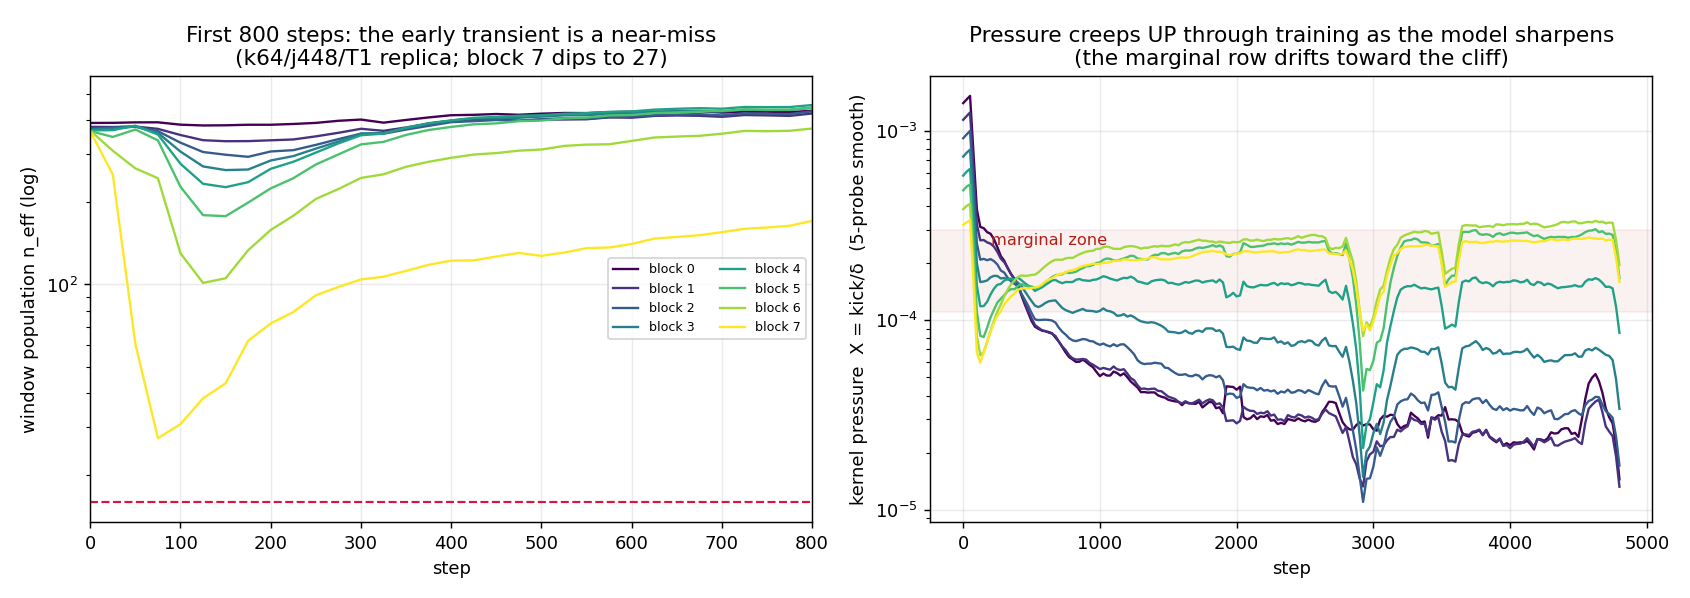
\includegraphics[width=\textwidth]{figures/kstab_probe5k_dip_creep.png}
\caption{
Gradient-resolved replica of \(K64,J448,T1\).
Left: early reduction of the effective kernel population.
Right: gradual increase of the pressure diagnostic during training.
}
\end{figure}

The gradient-resolved replica suggests two refinements.

\begin{itemize}[leftmargin=1.4em]

\item \textbf{The early training transient is a high-risk period.}

Within approximately the first 100 steps, the effective kernel population in
deep blocks drops strongly; for example, block 7 changes from approximately
363 to 27 while \(\chi\) initially reaches around \(10^{-3}\).

The methods that fail almost immediately---\(T=0.1\), detach, and
project---all fail during this phase.

Runs that remain stable first recover from this transient.

\item \textbf{Pressure can increase gradually later in training.}

After the early recovery, \(\chi\) rises again over time.
In block 7 it increases from approximately
\[
1.2\times10^{-4}
\]
to
\[
2.7\times10^{-4}
\]
by step 4800.

The main reason is that the score distribution sharpens:
\(\delta\) decreases faster than the surrogate kick decreases.

Thus late failures need not arise solely because the model waits for a rare
event at a fixed operating point.
The operating point itself can become progressively less stable.

\item \textbf{The relevant geometry differs substantially across layers.}

Blocks 5--7 occupy the marginal regime while blocks 0--4 relax toward lower
pressure.

This motivates controlling temperature separately by layer rather than with a
single model-wide scalar.

\end{itemize}

After wave 1, the main revision is therefore:

\begin{quote}
A marginal configuration should be viewed as having a nonzero, potentially
time-dependent failure rate, rather than as being guaranteed to diverge at a
particular step.
\end{quote}


% ============================================================
\section{Wave 2.0: the first controller was mis-calibrated}
% ============================================================

Approximately 800 steps into the first adaptive-temperature experiments,
telemetry showed that the kick-based trim was not calibrated correctly.

Healthy runs were reducing \(T\) aggressively; for example, the \(K=64\)
controller moved from approximately
\[
T=0.97
\]
to
\[
T=0.45,
\]
eventually operating near the population-floor intervention.

The source of the mismatch is that the measured
\[
|g_s|
\]
contains the task loss's per-token normalization.

The probe captures used to calibrate the target were computed with
approximately 256-token batches, while live training steps contain roughly
50k tokens.

Thus an absolute threshold expressed in task-gradient units changes with batch
normalization and does not transfer between the probe and training settings.

This invalidates the use of the original gradient-unit \(\chi\) as a portable
controller target.

The population floor itself remained useful:
the \(T_0=0.1\) rescue had already increased \(T\) to approximately 0.5 while
maintaining healthy loss, whereas the corresponding fixed-\(T=0.1\) run had
already failed.


% ============================================================
\section{A forward-only geometric pressure measure}
% ============================================================

To remove the dependence on gradient normalization, define

\[
\boxed{
\chigeo
=
\frac{b}
{2T\,\delta}
}.
\]

This quantity depends only on forward score geometry and is dimensionless.

At checkpoint 2000, using the maximum value across layers:

\begin{itemize}[leftmargin=1.4em]

\item every measured run with
\[
\chigeo\lesssim55
\]
survived;

\item every observed failure had
\[
\chigeo\gtrsim58;
\]

\item the \(K=64,T=1\) row sits around
\[
\chigeo\approx114,
\]
where outcome is strongly seed-dependent.
\end{itemize}

Within the measured runs, the additional \(u\)-dependent factor in the
gradient-based \(\chi\) provides relatively little discriminating information
beyond this score geometry.

The controller was therefore redesigned to target

\[
\chigeo
=
\frac{\EMA(b)}
{2T\,\EMA(\delta)}.
\]

The initial target was set to 45, slightly below the measured
\(K=32,T=1\) operating point of approximately 51.

Using measured
\[
\frac{b}{\delta}
\approx
80,\ 212,\ 319
\]
for
\[
K=32,\ 64,\ 96,
\]
the pre-registered expected temperatures were approximately:

\[
T\approx0.9\text{--}1.2
\qquad
(K=32),
\]

\[
T\approx2\text{--}2.6
\qquad
(K=64),
\]

\[
T\approx3\text{--}4
\qquad
(K=96).
\]

The purpose of this wave was to test whether a controller using only local
score geometry could recover the empirically safe temperature scale.


% ============================================================
\section{Wave 2.1 mid-flight results}
% ============================================================

At approximately step 2400:

\begin{center}\small
\begin{tabular}{lrrrrrl}
\toprule
run & \(T_0\) & \code{rb\_temp} @2.4k & \code{rb\_chi} & window & loss &
pre-registered \(T\) \\
\midrule

\code{k32\_j480\_servo}
&
1.0 & \textbf{0.947} & 46.4 & 129 & 1.919 &
0.9--1.2 \(\checkmark\)
\\

\code{k32\_j480\_t05\_servo}
&
0.5 & \textbf{0.946} & 37.2 & 143 & 1.942 &
rescue toward same operating point \(\checkmark\)
\\

\code{k32\_j96\_t01\_servo}
&
0.1 & \textbf{1.039} & 44.8 & 103 & 1.905 &
rescue from early-collapse regime \(\checkmark\)
\\

\code{k64\_j448\_servo}
&
1.0 & \textbf{2.268} & 45.0 & 450 & 1.884 &
2--2.6 \(\checkmark\)
\\

\code{k96\_j416\_servo}
&
1.0 & \textbf{3.001} & 45.5 & 483 & 1.908 &
3--4 \(\checkmark\)
\\

\bottomrule
\end{tabular}
\end{center}

The three \(K=32\) runs started from very different temperatures:
\[
1.0,\qquad0.5,\qquad0.1.
\]

By step 2400, all had converged to approximately
\[
0.95\text{--}1.04.
\]

Similarly, the \(K=64\) and \(K=96\) runs settled around
\[
2.27
\quad\text{and}\quad
3.00,
\]
respectively.

These values are approximately proportional to the previously measured
\[
b/\delta
=
80,\ 212,\ 319.
\]

Thus, at this stage of training, the geometric controller recovered the
expected \(K\)-dependent temperature scale without an explicit \(K\)-lookup
table.

In parallel,
\code{kstab\_k96\_j416\_t1}
with fixed \(T=1\) diverged by approximately step 3800, within the
pre-registered 1.5--6k interval.

This is an important out-of-sample test because \(K=96\) had not previously
been trained successfully in this setup, and the instability prediction was
made from score geometry measured before the run.


% ============================================================
\section{Wave 2.1 final results}
% ============================================================

\begin{center}\small
\begin{tabular}{p{4.4cm}p{3.6cm}rp{4.2cm}}
\toprule
run & outcome & final CE & reference \\
\midrule

\code{kstab\_k64\_j448\_servo}
&
stable
&
\textbf{1.4691}
&
fixed \(T=2\): 1.4724;
fixed \(T=1\): diverged at 3940
\\

\code{kstab\_k64\_j448\_servo\_s2}
&
stable
&
\textbf{1.4608}
&
best \(K=64\) result in the project
\\

\code{kstab\_k96\_j416\_servo}
&
stable
&
\textbf{1.4734}
&
fixed \(T=1\): diverged at 1640
\\

\code{kstab\_k32\_j480\_t05\_servo}
(\(T_0=0.5\))
&
stable; one recoverable burst near 8.9k
&
1.5075
&
fixed \(T=0.5\): diverged at 7760
\\

\code{kstab\_k32\_j96\_t01\_servo}
(\(T_0=0.1\))
&
stable; one recoverable burst near 5.1k; guard raised \(T\) to 2.2 during the
event
&
1.5261
&
fixed \(T=0.1\): diverged within 640 steps;
fixed \(T=1\), same \(J\): 1.525
\\

\textbf{\code{kstab\_k32\_j480\_servo}}
(\(T_0=1\), null test)
&
\died{destabilized at approximately 4140}
&
3.945
&
fixed \(T=1\): stable, 1.491
\\

\bottomrule
\end{tabular}
\end{center}


\begin{figure}[h]
\centering
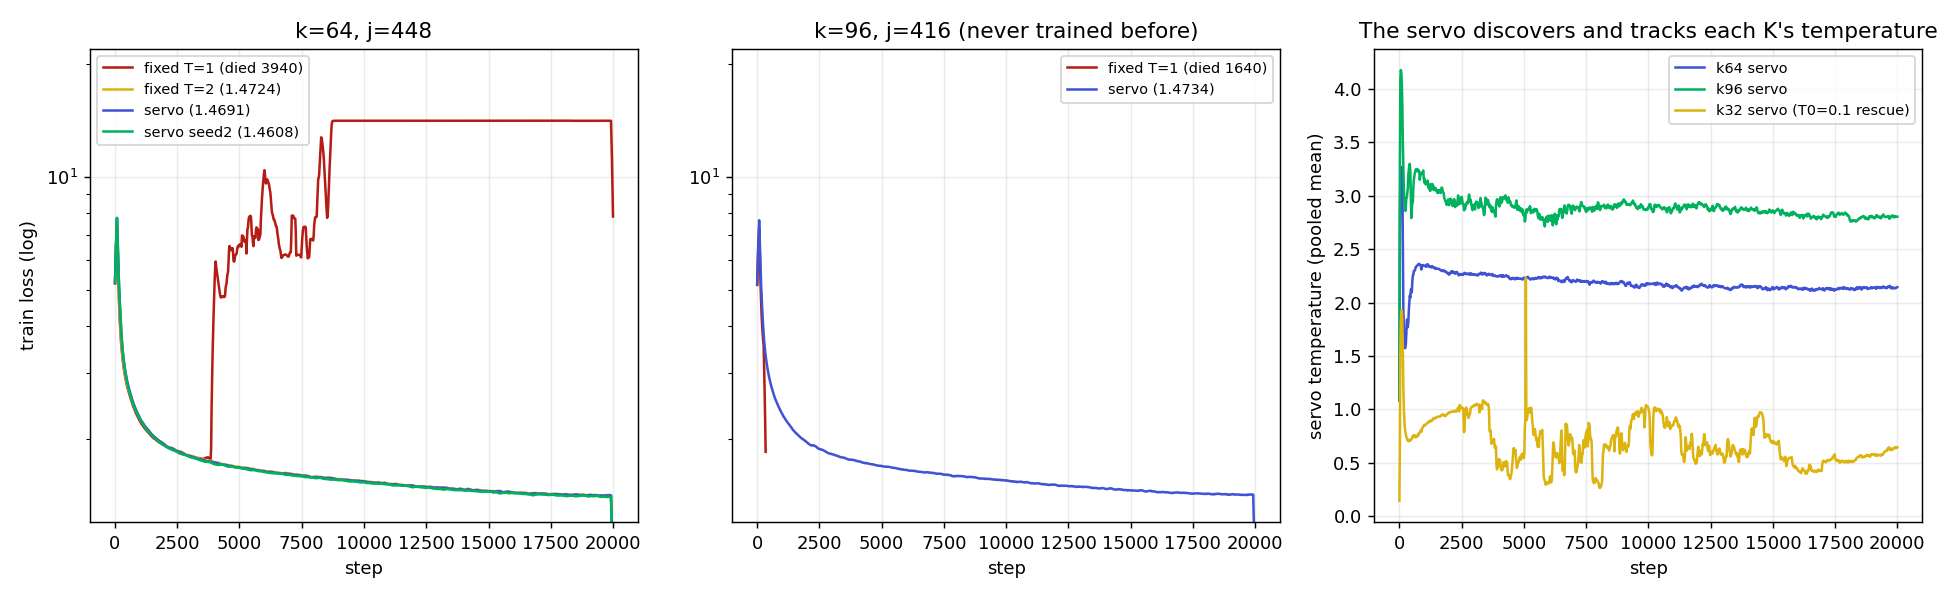
\includegraphics[width=\textwidth]{figures/kstab_servo_headline.png}
\caption{
Adaptive versus fixed temperature.
Left: \(K=64,\ J=448\).
Middle: \(K=96,\ J=416\).
Right: per-layer temperatures selected by the controller.
}
\end{figure}


% ============================================================
\section{Interpretation of the null-test failure}
% ============================================================

The failed \(K=32,J=480,T_0=1\) null test revealed a flaw in the symmetric
temperature controller.

The controller attempted to maintain
\[
\chigeo=45
\]
by moving \(T\) both upward and downward.

Between approximately steps 4k and 8k, it reduced \(T\) to the range
\[
0.49\text{--}0.70,
\]
which overlaps the empirically marginal \(T\approx0.5\text{--}0.75\) regime.

The reason is that the safe operating value of \(\chigeo\) is not constant
during training.

The stable fixed-\(T=1\), \(K=32\) reference run starts around
\[
\chigeo\approx39
\]
and gradually falls toward approximately 30.

Therefore forcing the model back toward 45 requires progressively decreasing
\(T\), even though the model is already in a stable regime.

The controller was consequently sharpening the kernel beyond a temperature
known to be safe.

In the failed null-test run, the boundary score increased for several thousand
steps before a late excursion reached
\[
b\approx2500
\]
and became unrecoverable.

The two \(K=32\) runs that began from initially unsafe temperatures happened to
survive, while the nominally safe null test failed after the controller moved
it into the marginal region.

This is consistent with the earlier observation that marginal operating points
have a stochastic failure rate rather than a deterministic outcome.


\begin{figure}[h]
\centering
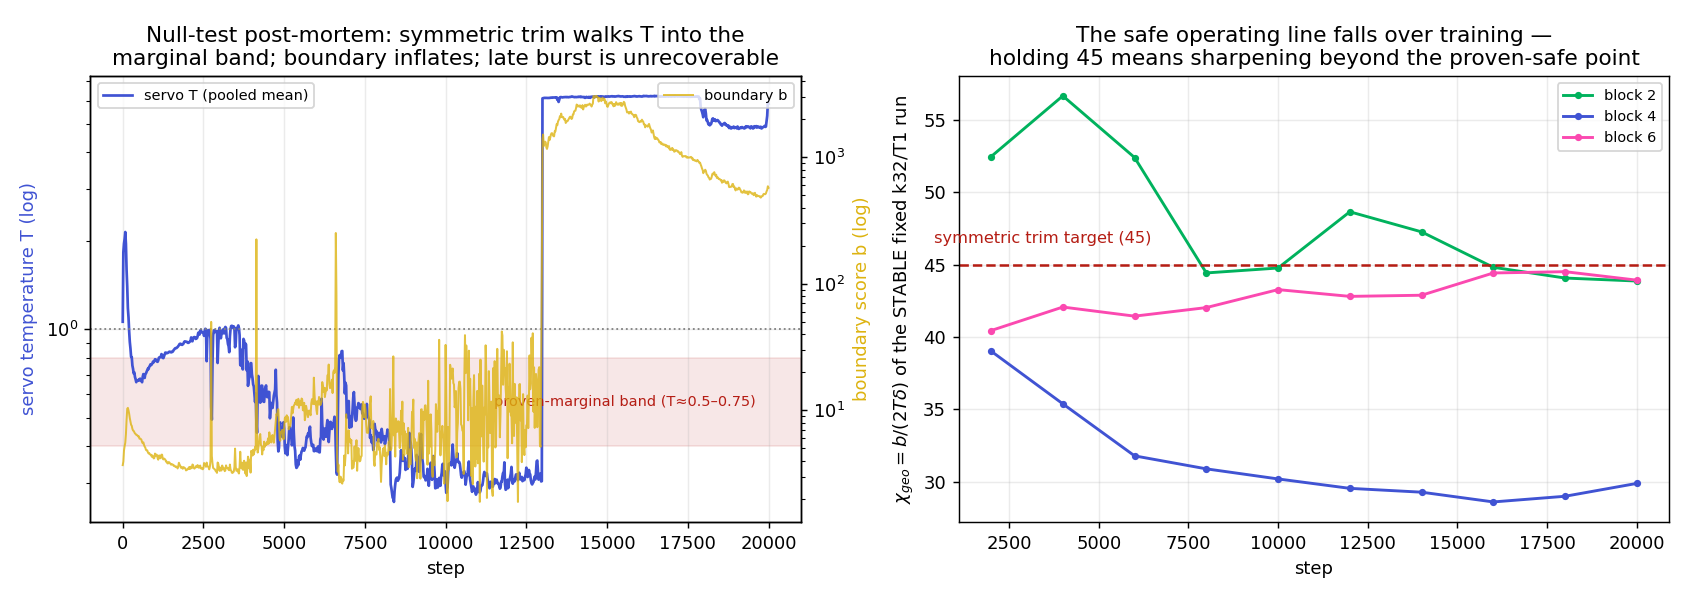
\includegraphics[width=\textwidth]{figures/kstab_nulltest_postmortem.png}
\caption{
Null-test analysis.
Left: the symmetric controller reduces \(T\) into the marginal regime before
the final boundary excursion.
Right: in the stable fixed-\(T=1\) \(K=32\) run,
\(\chigeo\) decreases naturally during training, so forcing it upward to a
fixed target unnecessarily sharpens the kernel.
}
\end{figure}


% ============================================================
\section{Controller revision: protective-only temperature adaptation}
% ============================================================

The controller has therefore been changed from a symmetric regulator to a
protective mechanism.

The revised rule imposes

\[
T
\ge
T_{\mathrm{configured}},
\]

where \(T_{\mathrm{configured}}\) is the baseline temperature supplied by the
experiment.

The controller may increase \(T\) when the measured geometry becomes unsafe,
but it does not decrease \(T\) below the baseline in an attempt to improve
sharpness or quality.

This asymmetry is motivated directly by the experiments:

\begin{itemize}[leftmargin=1.4em]

\item increasing \(T\) above the baseline prevents instability in the
high-pressure \(K=64\) and \(K=96\) regimes;

\item decreasing \(T\) below a known-safe baseline moves the model toward the
documented \(T=0.5\)--0.75 marginal region;

\item the fixed baseline already provides the desired quality in the
low-pressure regime, so there is limited justification for taking this
additional stability risk.
\end{itemize}

Wave 2.2 repeats the null test with this lower temperature bound using two
random seeds, together with a repeated \(K=96\) run.

% ============================================================
\section{Wave 2.2 results: the protective controller passes the null test}
% ============================================================

All three runs completed 20k steps with no destabilization onset.

\begin{center}\small
\begin{tabular}{p{4.6cm}p{3.0cm}rp{4.2cm}}
\toprule
run & outcome & final CE & reference \\
\midrule

\code{kstab\_k32\_j480\_servo} (null test, redone)
&
stable
&
\textbf{1.4879}
&
fixed \(T=1\): 1.4910;
symmetric controller: diverged at 4140
\\

\code{kstab\_k32\_j480\_servo\_s2}
&
stable
&
1.4957
&
seed repeat
\\

\code{kstab\_k96\_j416\_servo\_s2}
&
stable
&
\textbf{1.4665}
&
seed 1: 1.4734;
fixed \(T=1\): diverged at 1640
\\

\bottomrule
\end{tabular}
\end{center}

The protective lower bound resolves the one failure observed in wave 2.1.
The redone null test now slightly exceeds the fixed-\(T=1\) reference
quality, and the \(K=96\) result is reproduced across seeds.

After this revision, all eleven adaptive-temperature runs launched with the
protective controller or unaffected by the symmetric-trim flaw completed 20k
steps stably, across \(K=32,64,96\), two seeds, and starting temperatures
from 0.1 to 1.0, with final quality at or above the corresponding fixed-\(T\)
baselines.


% ============================================================
\section{Per-layer temperatures}
% ============================================================

The final checkpoints of the successful controller runs show substantial
layer-to-layer variation.

For \(K=64\), blocks 0 through 7 settle approximately at

\[
2.74,\ 2.48,\ 2.11,\ 1.83,\ 1.82,\ 1.99,\ 1.97,\ 2.21.
\]

The profile is roughly U-shaped across depth.

For \(K=96\), the same qualitative pattern appears at a larger overall scale,
approximately

\[
3.52,\ \ldots,\ 2.06,\ \ldots,\ 3.06.
\]

The temperature varies by about a factor of 1.5 within a single model.

This supports the earlier conclusion that the relevant score geometry is
layer-dependent and that a single global temperature is unlikely to be
optimal across all bottlenecks.


% ============================================================
\section{Current interpretation}
% ============================================================

The evidence currently supports the following picture.

\begin{enumerate}[leftmargin=1.6em]

\item
The instability is not explained by loss of the zero-sum property.
The kappa correction continues to remove the collective score-gradient mode
during unstable runs.

\item
The instability is strongly associated with the relationship between kernel
width and local score geometry.

Both decreasing \(T\) and increasing \(K\) can move the system into a regime
where the kernel is too sharp relative to the density of scores near the
support boundary.

\item
The \(K=32\to64\) instability and the \(T=1\to0.5\) instability are consistent
with the same mechanism.

The measured local score density quantitatively accounts for the approximate
factor-of-two change in the required temperature.

\item
Instability typically develops through changes in activation scale before
large changes in task loss become visible.

Boundary-score inflation is therefore a more sensitive early indicator than
CE.

\item
Marginal configurations exhibit transient inflation bursts.
Whether a particular trajectory eventually diverges is stochastic, and the
failure rate itself can increase over training as the score distribution
sharpens.

\item
A particularly dangerous state occurs when the effective kernel population
falls toward
\[
\neff=O(1).
\]
At that point the distributed correction approaches the single-boundary-feature
\code{through\_rank} limit.

\item
The purely geometric quantity
\[
\chigeo
=
\frac{b}{2T\delta}
\]
captures the relevant variation across the tested values of \(K\), \(T\), and
training time substantially better than an absolute gradient-unit threshold,
because it is independent of loss normalization.

\item
Adaptive temperature control is effective when used protectively:
increase \(T\) when local geometry becomes unsafe, but do not reduce it below a
known-safe configured baseline.

\end{enumerate}


% ============================================================
\section{Remaining uncertainties}
% ============================================================

Several aspects remain unresolved.

\begin{itemize}[leftmargin=1.4em]

\item
The precise mechanism that determines which run fails within a marginal
\((K,T)\) row is not fully explained.

For \(K=64,T=1\), burst rate increases with effective candidate population,
but the \(T=0.5\) row does not show the same ordering with \(J\).

\item
The proposed cumulative asymmetry in near-boundary feature motion is measurable
but small in healthy runs.

More direct evidence is still needed to determine exactly how this small bias
couples to global activation-scale growth.

\item
The role of the downstream architecture, particularly
\code{residual\_out}, deserves separate analysis.
Once scale growth becomes severe, the current architecture allows it to
propagate and amplify through depth, but this does not by itself identify the
initial cause of the instability.

\item
The empirical thresholds for \(\chigeo\) are based on the present architecture,
optimizer, and training setup.
The quantity is dimensionless and transfers better than the earlier
gradient-unit criterion, but the numerical safe range should not yet be
treated as universal.

\item
The protective controller has been validated on \(K=32,64,96\) in the current
campaign, but additional \(K\), architecture, and seed sweeps are required to
determine how broadly the rule generalizes.

\end{itemize}


% ============================================================
\section{Summary}
% ============================================================

The original question was why
\code{through\_rank\_kappa} can be stable and high-performing at
\(K=32,T=1\), yet fail when either \(K\) is increased or \(T\) is decreased.

The measurements support a common explanation.

The relevant control parameter is not \(K\) or \(T\) separately, but the
sharpness of the kernel relative to the local score spacing near the
\(K/(K+1)\) boundary.

Increasing \(K\) moves the boundary into a denser part of the score
distribution.
Reducing \(T\) sharpens the kernel.
Both therefore increase the pressure exerted on the near-boundary region.

At sufficiently high pressure, score-scale excursions become frequent.
A severe excursion can reduce the effective kernel population toward one,
at which point the distributed correction loses its main stabilizing
advantage and approaches the previously unstable single-boundary-feature
limit.

A forward-only diagnostic,

\[
\chigeo
=
\frac{b}{2T\delta},
\]

captures the observed \(K\)- and \(T\)-dependence and predicts the temperature
scale required at previously untested \(K\).

An adaptive, per-layer controller can use this geometry to increase \(T\) when
necessary.
The controller should be protective rather than symmetric: it may broaden the
kernel when the local geometry becomes unsafe, but should not sharpen the
kernel below a known-safe configured temperature merely to maintain a fixed
target value of \(\chigeo\).

\end{document}